\chapter{Thermodynamics}

\pagestyle{fancy}
\fancyhf{}
\fancyhead[OC]{\leftmark}
\fancyhead[EC]{\rightmark}
%\renewcommand{\footrulewidth}{1pt}
\cfoot{\thepage}

\section{Key concepts and formulae}
\begin{itemize}
    \item First Law of thermodynamics \\dQ = dU + dW
    
    \item Internal energy of an ideal gas \\U = nC$_v$T and dU = nC$_v$dT
    
    \item dQ = mcdT  where, \\m = mass of the substance \\c = Specific heat capacity of that substance \\dT = change in temperature
    
    \item 	$\Delta$S $\geq$ $\int \frac{dQ}{T}$ where, $\Delta$S = change in entropy and T = Temperature of the system.  \\Also, $\Delta S = \frac{\Delta Q}{T}$. 
    
    \item S = k ln(w) where,\\ k = Boltzmann constant\\ W = number of microscopic states of a system 
    
    \item	Ensure the temperature is in kelvin unit. 

    \item Find if something is conserved for example, no. of moles or molecules, internal energy, etc. 

    \item Check if the system is insulated or conducting. (close or open).
    
    \item \textbf{Sign Convention}: \\If the system gives away some heat then $\Delta$Q $<$ 0. \\ \\If the volume of the system contracts, work done by the gas or pressure is $\Delta$W $<$ 0. \\ \\This goes with the analogy of work done in mechanics. The pressure on the system boundary by the gas applies an outward force on the boundary and hence according to the choice of the directions of force and displacement vectors, we can determine whether the work is positive or negative. 
    
    \item \textbf{Dalton’s Law}: The total pressure exerted by a gas equals to the sum of the partial pressures.  P = P$_A$ + P$_B$ + ……., where P$_A$ is the pressure due to the molecules of type A and P$_B$ due to the molecules of type B and so on.  
    
    \item \textbf{Specific Heat Ratios}: \\	For monoatomic gases, $\gamma$ = 1.67 = $\frac{5}{3}$ \\For Diatomic gases, $\gamma$ = 1.4 = $\frac{7}{5}$ \\For Triatomic gases, $\gamma$ = 1.3 = $\frac{9}{7}$   \\We can also calculate Cp and Cv for each type of gases by using the relation C$_p$ = C$_v$ + R. 

\end{itemize}

\section{Level 1 Problems}
\begin{enumerate}
    \item At very low temperatures the heat capacity of crystals is equal to C = $a$T$^3$, where $a$ is a constant. Find the entropy of a crystal as a function of temperature in this temperature range. (IR 2.142)  \\\\
    \textbf{Hint}: \\
    Heat capacity (c) = $a$T$^3$ \\dQ  =  cdT \\$\Delta$S = $\int \frac{dQ}{T}$
    
    \item Find the entropy increment of an aluminum bar of mass m = 3.0 kg on its heating from the temperature T$_1$ = 300K up to T$_2$ = 600K if in this temperature range the specific heat capacity of aluminum varies as C = $a$ + $b$T, where $a$ = 0.77 J/(g.K), $b$ = 0.46 mJ/(g.K$^2$). \\\\
    \textbf{Solution}:\\
    mass(m) = 3 kg \\T$_1$ = 300K \\T$_2$ = 600K \\Specific heat capacity (c) = $a$ + $b$T , where $a$ = 0.77 J/(g.k), $b$ = 0.46 mJ/(g.k$^2$) \\\\
    Check the units of constants, convert them into reasonable units. \\
    $a$ = 0.77$\times$10$^3$ J (kg.k),   $b$ = 0.46 J/ (kg.k$^2$) 
    
    \begin{align*}
        \Delta S = \int_{T_1}^{T_2} \frac{dQ}{T} 
    \end{align*}
and we know, $dQ = m(a + bT)dT$

\begin{align*}
    &= \int_{T_1}^{T_2}\frac{m(a + bT)dT}{T}\\
    &= m\int_{T_1}^{T_2}\frac{adT}{T} + m\int_{T_1}^{T_2}\frac{bTdT}{T}\\
    &= m ln(T_2/T_1) + m b (T_2 - T_1)\\
    &= m[ln(T_2/T_1) + (T_2 - T_1)]\\
    &= 3\times770ln(2) + 3\times0.46(300)\\
    &= 2015.17 J/k 
\end{align*}

\item Calculate the value of $\gamma$ = Cp/Cv for a gaseous mixture of consisting of n$_1$ = 2.0 moles of oxygen and n$_2$ = 3.0 moles of carbon dioxide. The gases are assumed to be ideal. (IR 2.33)\\
\textbf{Solution}:
\begin{align*}
    \text{Moles of oxygen} (n_1) &= 2 \\
    \text{Moles of CO}{_2} (n_2) &= 3 \\
    \text{    Let }  \gamma_{mix}  \text{ be equal to }  C_{p,mix}/C_{v,mix} \\
    \text{Also, for the mixture total no. of moles is }n_1 + n_2.\\
    (n_1 + n_2) C_{v,mix}T &= n_1C_{v1}T + n_2C_{v2}T \\ \text{  [Each gas contributes to the total internal energy]}\\
    \therefore C_{v, mix} &= \frac{n_1C_{v1}T + n_2C_{v2}}{n_1 + n_2}\\
    \text{similarly, } (n_1 + n_2) C_{p,mix}T &= n_1 C_{p1}T + n_2C_{p2}T \\
    \therefore C_{p, mix} &= \frac{n_1 C_{p1} + n_2C_{p2}}{n_1 + n_2}\\
    \text{Hence, }\gamma_{mix} &= \frac{C_{p,mix}}{C_{v,mix}}\\
    &= \frac{n_1 C_{p1} + n_2C_{p2}}{n_1C_{v1}T + n_2C_{v2}}\\
    &= \frac{\frac{n_1 \gamma_1}{\gamma_1 -1}+ \frac{n_2 \gamma_2}{\gamma_2 - 1}}{\frac{n_1}{\gamma_1 -1} + \frac{n_2}{\gamma_2 - 1}}\\
    &= \frac{n_1\gamma_1(\gamma_2 - 1) + n_2\gamma_2(\gamma_1 - 1)}{n_1(\gamma_2 - 1) + n_2(\gamma_1 - 1)}
\end{align*}

    \item Consider two identical iron spheres(fig 3.1), one of which lies on a thermally insulated plate, whilst the other hangs from an insulating thread. Equal amount of energies was given to both, which one will have higher temperature? (200 Puzzling Problems)\\
    \begin{figure}[htp]
        \centering
        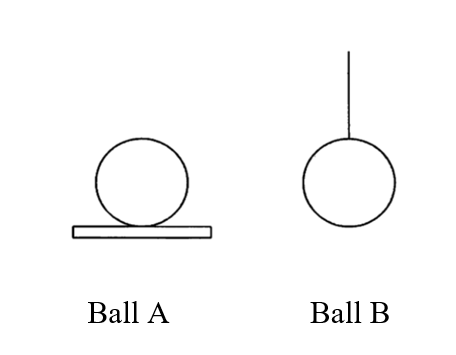
\includegraphics{mainmatter/thermo3.1.PNG}
        \caption{}
        \label{fig:thermo3.1}
    \end{figure}
\\
\textbf{Solution}:\\
    For equal amount of heat supplied to each ball, the balls will expand. For the ball B the center of gravity(CoG) will lower and for ball A the CoG will rise up. \\
    For the ball B the potential energy will be converted into heat energy as the CoG lowers, but for ball A some heat energy is spent in the form of potential energy to raise the CoG. Hence, ball B will have a slightly greater temperature than ball A.

\item What is the change in entropy that occurs when two moles of helium and three moles of oxygen, both at s.t.p. (T = 273 K, and P = 1.01 $\times$ 10$^5$ Pa) and in adjacent volumes, are allowed to mix by removing the partition between them? \\
\begin{figure}[htp]
    \centering
    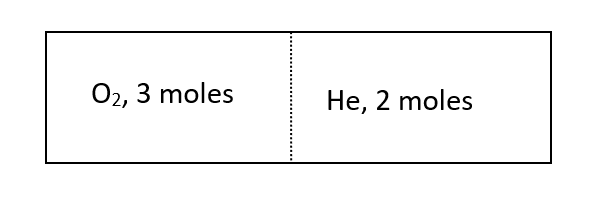
\includegraphics{mainmatter/thermo3.2.PNG}
    \caption{}
    \label{fig:thermo3.2}
\end{figure}
\\
\textbf{Solution}:\\
Since both the compartments have the same condition, no change in temperature and pressure will occur. \\
For constant temperature and pressure, volume(V) $\propto$ no. of moles (n).\\ 
And, let the total volume of the container be 5V, so that volume of oxygen is 3V and that of helium is 2V. \\
The total change in entropy is equal to:
$\Delta S_{tot}$ $=$ $\Delta$$S_{o_2}$ $+$ $\Delta S_{He}$\\\\
Note: Remember the entropy in this problem is addressing the no. of microscopic states of gas.\\
For O$_2$, \\
\begin{align*}
    \Delta S_{o_2}
    &= kln\left(\frac{w_f}{w_i}\right)\\
    &= kln\left(\frac{5V}{3V}\right)^{3N_A}\\
\end{align*}
We know W $\propto$ (volume)$^\text{no. of molecules}$, where W is the total no. of possible microscopic states. Hence, $w_f$ is the final no. of microscopic states and $w_i$ is the initial no. of microscopic states.\\\\
Now, for He, \\
\begin{align*}
    \Delta S_{He} = kln\left(\frac{5V}{2V}\right)^{2N_A}
\end{align*}
Hence, 
\begin{align*}
    \Delta S &= kln\left(\frac{5V}{3V}\right)^{3N_A} + kln\left(\frac{5V}{2V}\right)^{2N_A}\\
    &=  3N_A k ln(5/3) + 2N_A k ln(5/2)
\end{align*}\\
Putting back the values of N$_A$ and K, we get $\Delta S = 27.9 JK^{-1}$. 

\item A hot-air balloon stays aloft because hot air at atmospheric pressure is less dense than cooler air at the same pressure. If the volume of the balloon is 500.0 $m^3$ and the surrounding air is at 15.0$^{\degree}$C, what must the temperature of the air in the balloon be for it to lift a total load of 290 kg (in addition to the mass of the hot air)? The density of air at 15.0$^{\degree}$C and atmospheric pressure is 1.23 kg/m$^3$. (UP 18.55) \\
\textbf{\begin{figure}[htp]
    \centering
    
\includegraphics{mainmatter/thermo3.3.PNG}
    \caption{}
    \label{fig:thermo3.2}
\end{figure}}\\
\textbf{Soultion}: \\
Volume of the balloon (V) = 500 m$^3$\\
Surrounding temperature (T$_s$) = 15$^{\degree}$C \\
Mass of the load (m) = 290 kg \\
Density of the air at 15$^{\degree}$C and atmospheric Pressure ($\rho _s$) = 1.23 kg/m$^3$\\\\
We need to find the temperature of the air inside the balloon (T$_i$). \\\\
We know, from Archimedes' Principle, the buoyant force on the balloon(F) = V$\rho _s$g, where V is the volume of the displaced air. \\\\
The total weight to be lifted is\\
= mg + Mg [M is the mass of the hot air inside the balloon]\\
= mg + $\rho _i$Vg [$\rho _i$ is the density of the air inside the balloon]\\
\begin{align*}
    PV &= nRT\\
    &=\ddfrac{m}{M}RT \text{, which implies } \rho T = \text{cont.}\\
    \text{Hence, }\\
    \rho_s T_s &= \rho_i T_i\\
    \text{The total weight becomes, }\\
    mg + Vg\left(\frac{\rho_s T_s}{T_i}\right)\\
    \text{equating the buoyant force and the weight, }\\
    V\rho_sg &= mg + Vg\left(\frac{\rho_s T_s}{T_i}\right)\\
    \text{or, }V\rho_s - m &= V\left(\frac{\rho_s T_s}{T_i}\right)\\
    \text{or, }T_i &= \frac{V\rho_s T_s}{V\rho_s - m}\\\\
    \text{Putting back the given values, } T_i = 545K \text{ or }272^{\degree} C. 
\end{align*}

\item A typical dorm room or bedroom contains about 2500 moles of air. Find the change in the internal energy of this much air when it is cooled from 35.0$\degree$C to 26.0$\degree$C at a constant pressure of 1.00 atm. Treat the air as an ideal gas with $\gamma$ = 1.400 (UP). \\\\
\textbf{Hint}:\\
\begin{align*}
    dU &= nC_vdT \text{ and, }\\
    C_v &= \frac{R}{\gamma - 1}
\end{align*}

\item 	Vessel 1 and vessel 2 contain n = 1.2 moles of gaseous helium. The ratio of the vessels’ volumes V$_2$/V$_1$ = $\alpha$ = 2.0 and the ratio of the absolute temperatures of helium in them T$_1$/T$_2$ = b = 1.5. Assuming the gas to be equal, find the difference of the gas entropies in these vessels, S$_2$ $-$ S$_1$.  (Irodov  2.135)\\
\textbf{Ans}: S$_2$ $-$ S$_1$ = $\gamma$R $\left(ln\alpha -  \frac{ln\beta}{\gamma -1}\right)$ = 1.0 J/K

\item 	At very low temperatures the molar heat capacity of rock salt varies with temperature according to Debye’s T$^3$ law: C = $K$$\frac{T^3}{\Theta^3}$ where $K$ = 1940 J/mol$\cdot$K  and $\Theta$ = 281 K.\\
(a) How much heat is required to raise the temperature of 1.50 mol of rock salt from 10.0 K to 40.0 K? (Hint: Use dQ = nCdT  and integrate.)\textbf{Ans: } 83.6 J\\
(b) What is the average molar heat capacity in this range? \textbf{Ans: }1.86 J/mol$\cdot$K\\
(c) What is the true molar heat capacity at 40.0 K? \textbf{Ans: }5.60 J/mol$\cdot$K\\
\textbf{(UP)}

\item A gas expands adiabatically and reversibly. What is its change in entropy? (UP)

\item Suppose 1.00 kg of water at 100$\degree$C is placed in thermal contact with 1.00 kg of water at 0$\degree$C. What is the total change in entropy? Assume that the specific heat of water is constant at 4190 J/Kg$\cdot$K over this temperature range. \textbf{(UP)}

\end{enumerate}
\section{Level 2 Problems and Solutions}
\begin{enumerate}
    \item An insulated container of negligible mass holds 0.600 kg of water at 45.0$\degree$C. You put a 0.0500-kg ice cube at $-15.0 \degree$C in the water. (a) Calculate the final temperature of the water once the ice has melted. (b) Calculate the change in entropy of the system. (UP)\\
    \textbf{\begin{figure}[htp]
    \centering
    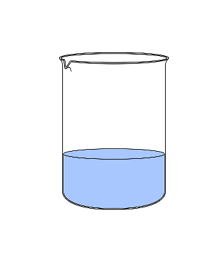
\includegraphics{mainmatter/thermo3.4.PNG}
    \caption{}
    \label{fig:thermo3.4}
\end{figure}}\\
    \textbf{Solution}:
    \begin{align*}
        \text{Given condition:}\\
        \text{Mass of water} (M_w) &= 0.6 \text{kg} \\
        \text{Initial temperature of water} (T_{i,w}) &= 45\degree C\\ 
        \text{Mass of Ice} (M_{ice}) &= 0.05 \text{kg}\\
        \text{Initial temperature of ice} (T_{i,ice}) &= -15\degree C
    \end{align*}
For ice at $-15\degree$C, we have to first check if the water contains enough heat to melt all the ice. So let's calculate the heat required to cool the ice from $-15\degree$C to 0$\degree$C.
\begin{align*}
    Q_1 &= M_{ice}C_{ice}\Delta T_{ice}\\  
     &= 0.05\times2100\times15 \\
     &= 1575 J 
\end{align*}
Also, calculate the amount of heat in the water.
\begin{align*}
    &= M_w C_w \Delta T_w\\
    &= 0.6\times4200\times45\\
    &= 113400 J 
\end{align*}
Hence, we see that water has enough heat to cool the ice to 0$\degree$C. Let’s check further if the amount of heat in the water is enough to change the ice at 0$\degree$C to water at 0$\degree$C.

\begin{align*}
    Q_2 &= M_{ice}L_f\\
     &= 0.05 \times 3.34 \times 10^5 \\
     &= 16700 J 
\end{align*}
We see that the water has enough heat to convert the ice into water. And since a lot of heat still remains in the water, there will be a resultant temperature T greater than 0$\degree$C. Using the energy conservation principle, we get: \\
\textbf{Note}: We can only use energy conservation principle for isolated systems.
\begin{align*}
    M_wC_w(T_w - T) &=  Q_1 + Q_2 + M_{ice}C_{ice}T\\
    \text{or, }2520 (45 – T)  &=  1575 + 16700 + 210T \\
    \text{or, }95125  &=  2730T\\
    \therefore T &= 34.84\degree C
\end{align*}
b)Now for entropy change, we know: \\
\begin{align*}
    \Delta S &= \Delta S_{ice} + \Delta S_{water}\\
\end{align*}  \\
Note: Convert the temperature units to Kelvin. Make sure you are using the correct temperature units.\\
Entropy change for ice:\\
\textbf{Entropy change of ice}(from -15$\degree$C to 0$\degree$C) + \textbf{entropy change of ice at 0$\degree$C to water at 0$\degree$C} + \textbf{entropy change of water at 0$\degree$C to water at 34.84$\degree$C}. 
\begin{align*}
    \Delta S_{ice}  &=  \int_{258K}^{273K} \frac{dQ}{T}   +   \frac{\Delta Q}{T}_\text{at T = 273K}   +   \int_{273K}^{307.84K} \frac{dQ}{T}\\
    &= M_{ice}C_{ice}\int_{258K}^{273K} \frac{dT}{T} + \frac{M_{ice}L_f}{T}_\text{at T = 273K} + M_{ice}C_{w}\int_{273K}^{307.84K} \frac{dT}{T}\\
    &=0.05\times2100\times ln\left(\frac{273}{258}\right) +\frac{0.05 \times 3.34 \times 10^5}{273} + 0.05\times 4200\times ln\left(\frac{307.84}{273}\right)\\
    &=92.33 J/K  
\end{align*}
Now, for water: \\
\begin{align*}
    \Delta S_{w} &= \int_{307.84K}^{318K} \frac{dQ}{T}\\
    &=M_{w}C_{w}\int_{307.84K}^{318K} \frac{dT}{T}\\
    &= 0.6\times4200\times ln\left(\frac{307.84}{318}\right)\\
    &= -81.82 J/K
\end{align*}
Hence, $\Delta$S = $\Delta$S$_{ice}$ + $\Delta$S$_w$ = 92.33 J/K - 81.82 J/K = 10.51 J/K. 
\\
\item The piston of mass M, which encloses the volume V$_o$ of a monoatomic gas under pressure P$_o$ and temperature T$_o$ moves at speed u. Determine the temperature and gas volume during the maximum compression. The system is thermally insulated. Neglecting the heat capacities of the plunger and the container. (CoPhO)\\\\
\textbf{Solution}:\\
\textbf{\begin{figure}[htp]
    \centering
    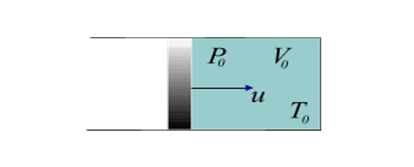
\includegraphics{mainmatter/thermo3.5.PNG}
    \caption{}
    \label{fig:thermo3.5}
\end{figure}}\\
The system is thermally insulated and the heat capacities of container and plunger are negligible. 
The kinetic energy of the piston will transform into internal energy of the gas at the maximum compression. 
\begin{align*}
    \frac{1}{2}Mu^2 &= nC_v \Delta T\\
    \text{or, }Mu^2 &= \frac{2nR(T - T_o)}{(\gamma - 1)}\\
    \text{or, } Mu^2 &=  \frac{2P_o V_o (T-T_o)}{T_o (\gamma - 1)}
\end{align*}
\textbf{Note: }PV = nRT, so nR = PV/T
\begin{align*}
    \therefore T &= \frac{Mu^2T_o(\gamma - 1)}{2P_o V_o} + T_o
\end{align*}
Also, since no heat is entering or escaping from the system, the process is adiabatic. We know that for adiabatic process: \\
\begin{align}
    P_oV_0 ^\gamma &=  PV^\gamma\\
    PV &= nRT 
\end{align}
Combining eqn 3.1 and 3.2, we get: 
\begin{align*}
    \frac{P_oV_o ^\gamma}{V^\gamma}V &= nRT \\
    \text{or, }\frac{P_oV_o ^\gamma}{V^\gamma}V &= \frac{P_o V_o}{T_o}T\\
    \text{or, }\left(\frac{V_o}{V}\right)^{\gamma -1} &= \frac{T}{T_o}\\
    \text{or, }\frac{V}{V_o} &= \left(\frac{T_o}{T}\right)^\frac{1}{\gamma -1}\\\\
    \therefore V = V_o\left(\frac{T_o}{T}\right)^\frac{1}{\gamma -1} 
\end{align*}
Substitute T from earlier calculation.

\item An ideal gas of molar mass M is contained in a very tall vertical cylindrical vessel in the uniform gravitational field in which free-fall acceleration equals g. Assuming the gas temperature to be the same and equal to T, find the height at which the center of gravity of the gas is located. (Irodov 2.18)\\\\
\textbf{Solution}: \\
Molar mass of the gas = M\\
gravitational field is uniform so, ‘g’ is constant. \\
Gas temperature is constant and is equal to ‘T’. \\
Now, 
\begin{align}
    PV &= nRT \nonumber\\
    \text{or, } PV &= \frac{m}{M} RT \nonumber\\
    \text{or, } p &= \frac{\rho RT}{M}
\end{align}
Also,(include figure for clarification)
\begin{align}
    dP &=  -\rho gdh 
\end{align}
from eqn. 3.3 and 3.4 we get, 
\begin{align*}
    P &= - dP\frac{RT}{Mgdh}\\
    \text{or, }\frac{dP}{P} &= - \frac{Mgdh}{RT}\\
    \text{or, }P &= P_o e^{-\frac{Mgh}{RT}}
\end{align*}
Since $\rho$ $\propto$ P, 
\begin{align*}
    \rho = \rho_oe^{-\frac{Mgh}{RT}}    
\end{align*}
Now for finding CoG, 
\begin{align*}
    H_{C.o.G} &=  \frac{\int_{0}^{\infty}{h dm}}{\int_{0}^{\infty}dm}\\
    &=  \frac{\int_{0}^{\infty}h\rho Adh}{\int_{0}^{\infty}\rho Adh}\\
    &= \frac{\int_{0}^{\infty}{he^{-\ \frac{Mgh}{RT}}dh}}{\int_{0}^{\infty}{e^{-\ \frac{Mgh}{RT}}dh}}\\
    &=  \frac{RT}{Mg}
\end{align*}
\end{enumerate}
\section{IPhO Problems and Solution}
\section{Supplementary Questions}
\begin{enumerate}
    \item A piece of copper of mass m = 90g at a temperature T$_1$ = 90{$\degree$}C was placed in a calorimeter in which ice of mass 50g was at a temperature -3{$\degree$}C. Find the entropy increment of the piece of copper by the moment the thermal equilibrium is reached. (Irodov 2.215).\\
    
    \item A worker pours 1.250 kg of molten lead at a temperature of 327.3 $\degree$C into 0.5000 kg of water at a temperature of 75$\degree$C in an insulated bucket of negligible mass. Assuming no heat loss to the surroundings, calculate the mass of lead and water remaining in the bucket when the materials have reached thermal equilibrium. (UP)\\
    

\item The atmosphere could be considered as ideal gas at constant temperature T = 300 K. The mass per mole of ‘air’ molecule is m = 0.029 kg. The gas constant is R = 8.31 J/(K$\cdot$mol).\\

a) For stationary atmosphere, set up a differential equation that relates the pressure p(h) at height h with the gravity acceleration g, the atmosphere mole number density $\rho$(h), and mass per mole m.\\

b)	Using the ideal gas law and the result in (a), set up a differential equation for the pressure p(h) as a function of height h.\\

c) Assuming P$_0$ is the pressure at h = 0, solve the differential equation in (b), and find the height where the pressure is $\frac{P_o}{2}$. (Hint: $\int\frac{dx}{x}$ = lnx )

\item What is the change in entropy occurs when two moles of helium and three moles of oxygen, both at s.t.p. (T = 273 K, and P = 1.01 $\times 10^5$ Pa) and in adjacent volumes, are allowed to mix by removing the partition between them? 

\item 
\end{enumerate}